\newpage
\part{Some More Advanced Considerations}\label{advanced} %%%%%%%%%%%%%%%

In the previous part, we saw what everyone should know about D templates. But in fact, there is much more to them than that. What follows is not necessarily more complicated, but it's probably a little less commonly used. As this document matures, some subjects may flow from \autoref{basics} into \autoref{advanced} and the other way round.

\section{Constraints}\label{constraints}

Templates constraints\index{template!constraints} are a way to block a template instantiation if some condition is not met. Any condition that can be determined at compile-time is authorized, which makes constraints a superset of templates specializations\index{template!specialization} (see \ref{specializations}). As such, their usage grew rapidly once they were introduced and, if Phobos\index{Phobos} is any indication, templates specializations are on the contrary becoming less common.

\subsection{Syntax}\label{constraintssyntax}

To obtain a constraint, put an \D{if} clause just after the template parameter list, and before the enclosed scope\index{scope!constraint}:

\index{syntax!templates constraints}
\begin{dcode}
template templateName(T,U,V) if (someCondition on T, U or V)
{
   ...
}
\end{dcode}

When the compiler tries to instantiate a template, if will first check the constraint. If it evaluates to \D{false}, the template declaration is not part of the considered set. That way, using constraints, you can keep or drop templates at your leasure. \D{is} expressions\index{is expression@\D{is} expression} are your friend there, allowing you to get compile-time introspection\index{compile-time!introspection} on types. See the appendix (\ref{isexpression}) for a crash course on it. 

You may have many template declarations with the same name and differing constraints (in fact, that's the very use case for constraints). Depending on the activated constraints, some or all will be considered by the compiler.

\index{template!constraints}
\begin{dcode}
module constrained;

template Constrained(T) 
    if (is(T : int)) { /*...*/ } // #1
template Constrained(T) 
    if (is(T : string)) { /*...*/ } // #2
template Constrained(T,U) 
    if (is(T : int) && !is(U : float)) { /*...*/ } // #3
template Constrained(T,U) 
    if (is(T : int) && is(U : float)) { /*...*/ } // #4

alias Constrained!(int) C1;      // #1
// alias Constrained!(string) C2; // Error, no declaration fits (string)
alias Constrained!(int,string) C3;// #3 and #4 considered, but #4 is dropped.
                                  // So #3 it is.
\end{dcode}

This syntax is the same for the special-cases templates seen in sections \ref{functiontemplates}, \ref{structtemplates}, \ref{classtemplates} and \ref{othertemplates}. The only tricky part is for class templates, where you may wonder where to put the constraint: before or after the inheritance list? The answer is: before.

\index{syntax!template constraints!for class templates}
\begin{dcode}
module constraintsyntax;

T theFunction(T)(T argument)
    if (is(T : int) || is(T : double)) 
{ return argument; }

struct TheStruct(T) 
    if (is(T : int) || is(T : double)) 
{ /*...*/ }

class TheClass(T) 
    if (is(T : int) || is(T : double)) 
    : BaseClass!T, Interface1 
{ /*...*/ }
\end{dcode}

When you write constraints, just remember they are a compile-time construct. For \DD{theFunction}, \DD{argument} is not known at compile-time, only its type, \DD{T}. Do not use \DD{argument} in your constraint. If you need a value of type \DD{T}, use \DD{T.init}. For example:

\index{template!constraints}
\begin{dcode}
module ctvalue;

auto callTwice(alias fun, T)(T arg)
    // Is it OK to do fun(fun(some T))?
    if (is(typeof({ 
                      fun(fun(T.init)); 
                  }()))) 
{
    return fun(fun(arg));
}
\end{dcode}

\subsection{Constraints Usage}\label{constraintsusage}

Constraints come from the same idea than C++0x\index{C++!C++0x} \DD{concept}, er\ldots, concept, although simpler to define, understand and, as shown by D, implement. The idea is to define a set of conditions a type must respect to be a representative of a `concept', and check for it before instantiating.

Have a look at constraints poster-child: \emph{ranges}\index{range}.\footnote{ Ranges are overdue a tutorial.} They were rapidly described in section \ref{functionflatten}.

\std{range} defines a set of templates\index{predicate templates!for ranges} that check the different ranges concepts, called \DD{isInputRange}, \DD{isForwardRange}\ldots I call these \D{bool}-becoming templates \emph{predicate templates} and talk about them in section \ref{predicates}. Usage is quite simple:

\index{predicate templates}
\index{range templates}
\begin{dcode}
module rangewrapper;
import std.range;

struct RangeWrapper(Range) 
    // Does Range comply with the input range 'concept'?
    if (isInputRange!Range) 
{ 
   /* Here we know that Range has at least three member functions:
      .front(), .popFront() and .empty(). We can use them happily.*/
}

// In the factory function too.
auto rangeWrapper(Range)(Range range) if (isInputRange!Range) 
{
    return RangeWrapper!(Range)(range);
}
\end{dcode}

In fact, it's a bit like a sort of compile-time interface or compile-time duck-typing: we do \emph{not} care about \DD{Range}'s `kind': it may by a \D{struct} or a \D{class} for all we know. What is important is that it respects the \emph{input range} concept.

The good news is that the compiler will complain\footnote{ I think \emph{compiler} and \emph{complain} must have the same root.} when it cannot instantiate a template due to constraints being not respected. It gives better error messages this way (although not as good as you might need).

\subsection{Constraints Limits}\label{constraintslimits}

The main problem is that, compared to templates specializations, you cannot do:

\index{template!constraints!limitations}
\begin{dcode}
module constraints_error;

template Temp(T) 
if (is(T:int))   // #1, specialized for ints
{ /*...*/ }

template Temp(T) // #2, generic case 
{ /*...*/ }

alias Temp!int TI;// Error!
\end{dcode}

Why an error? Because the compiler finds that both the \D{int}-specialized and the generic version can be instantiated. It cannot decide which one you mean and, quite correctly, does nothing, humble code that it is. No problem, says you, we will just add a constraint to the generic version:

\begin{dcode}
template Temp(T) if (is(T:int)) // #1
{ ... } // specialized for ints

template Temp(T) if (!is(T:int))// #2
{ ... } // generic case

Temp!int // Works!
\end{dcode}

Now, when you try to instantiate with an \D{int}, template \#2 is not present (its constraint is false and was dropped from the considered template list) and we can have \#1. Hurrah? Not quite. The \#1-constraint wormed its way into the generic version, adding code where none was initially. Imagine you had not one, but three different specialized versions:

\begin{dcode}
template Temp(T) if (is(T:int[])) // #1a
{ ... } // specialized for arrays of ints

template Temp(T) if (isRange!T) // #1b
{ ... } // specialized for ranges

template Temp(T) if (is(T:double[n], int n)) // #1c
{ ... } // specialized for static arrays of double

template Temp(T) // #2, generic
   if ( /* What constraint? */
{ ... }
\end{dcode}

OK, quick: what constraint for \#2? The complement to \emph{all} other constraints. See:

\begin{dcode}
template Temp(T) // #2, generic
   if ( !(is(T:int[]))
     && !isRange!T
     && !is(T:double[n], int n))
{ ... }
\end{dcode}

That's becoming complicated to maintain. If someone else adds a fourth specialization, you need to add a fourth inverted version of its constraint. Too bad, you still compile and calls \DD{Temp}: \DD{Temp!(}\D{int}\DD{[])}. And there: error! Why? Because constraints \#1a and \#1b are not mutually exclusive: an \D{int}\DD{[]} is also a input range. Which means that for \#1b, you need to add a clause excluding arrays of \D{int} and maybe modify constraint \#2.

Ouch. 

So, yes, constraints are wonderful, but they do have drawbacks. As a data point, this author uses them all the time, even though specializations (\ref{specializations}) are sometimes more user-friendly: most of what I want to impose and check on my types cannot be done by specializations. 

\subsection{Constraints, Specializations and \D{static if}:}
\label{constraintsorspecializations}

I mean, come on! Three different ways to decide if your template exists or not? 

\begin{dcode}
template Specialized(T : U[], U)
{ ... }

template Constrained(T) if (is(T : U[], U))
{ ... }

template StaticIfied(T)
{
    static if (is(T : U[], U))
    { ... }
    else // stop compilation
        static assert(0, "StaticIfied cannot be instantiated.");
}
\end{dcode}

What were the D designers thinking? Well, they got specializations (\ref{specializations}) from D's cousin, C++\index{C++}. The two other subsystems were added a few years later, as the power of D compile-time metaprogramming\index{compile-time!introspection} became apparent and more powerful tools were needed. So, the 'modern' subsystems are constraints and \D{static if} (\ref{staticif})\index{static if@\D{static if}}. Constraints are much more powerful than specializations, as anything you can test with specialization, you can test with an \D{is} expression in a constraint\index{is expression@\D{is} expression!in a constraint}. And \D{static if} is wonderfully useful outside of template instantiation, so these two are well implanted in D and are there to stay.
What about specializations, now? First, they are quite nice to have when porting some C++\index{C++} code. Second, they have a nice effet that constraints do \emph{not} have: when more than one definition could be instantiated, priority is given to the more specialized. You saw the explanation in the previous subsection.

So in the end, the conclusion is a bit of \emph{D Zen}\index{D Zen}: you are given tools, powerful tools. As these are powerful, they sometimes can do what other options in your toolbox can do also. D does not constrain (!) you, chose wisely.

\section{Predicate Templates}\label{predicates}

When you find yourself typing again and again the same \D{is} expression\index{is expression@\D{is} expression} or the same complicated constraint\index{template!constraints}, it's time to abstract it into another template, a \D{bool}-becoming one.\index{predicate templates} If you have a look a section \ref{istype}, you'll see a way to test if a particular piece of D code is OK (compilable) or not. Another way to obtain this is by using \D{\_\_traits}\DD{(compiles, some Code)}\index{\_\_traits@\D{\_\_traits}}.

In \autoref{examples}, the section \ref{staticfilter}, on page \pageref{graphcheck} shows another example of a predicate template.

\subsection{Testing for a member}

For example, if you want to test is some type can be serialized, through a \D{size\_t}\DD{ serialize()} member function:

\index{predicate templates!member testing}
\begin{dcode}
module isserializable;

template isSerialazable(Type)
{
    static if (__traits(compiles, {
                                   Type type;
                                   size_t num = type.serialize;
                                  }))
        enum bool isSerialazable = true;
    else
        enum bool isSerialazable = false;
}
\end{dcode}

\subsection{Testing for operations}

As seen in previous sections (\ref{structflatten}, \ref{constraintsusage}), we are writing here a kind of compile-time interface. Any type can pass this test, as long as it has a \DD{.serialize} member that returns a \D{size\_t}. Of course, you're not limited to testing member functions. Here is a template that verify some type has arithmetic operations:

\index{predicate templates!operator testing}
\begin{dcode}
module hasarithmeticoperations;

template hasArithmeticOperations(Type)
{
    static if (__traits(compiles, 
                       {   
                           Type t, result;
                           result = t + t; // addition
                           result = t - t; // substraction
                           result = t * t; // multiplication
                           result = t / t; // division
                           result = +t;    // unary +
                           result = -t;    // unary -
                       }))
        enum bool hasArithmeticOperations = true;
    else
        enum bool hasArithmeticOperations = false;
}

static assert(hasArithmeticOperations!int);
static assert(hasArithmeticOperations!double);

struct S {}
static assert(!hasArithmeticOperations!S);
\end{dcode}

As you can see, you can test for any type of D code, which means it's \emph{much} more powerful than templates specializations (\ref{specializations}\index{template!specialization!compared to constraints}) or the \D{is} expression (Appendix \ref{isexpression})\index{is expression@\D{is} expression!compared to constraints}.

You may also get a certain feel of a... \emph{pattern} emerging from the previous two examples. All the scaffolding, the boilerplate, is the same. And we could easily template it on what operator to test, for example. It's possible to do that, but it means crafting code at compile-time. Wait until you see string mixins\index{string mixins} (\ref{stringmixins}) and CTFE\index{CTFE} (\ref{ctfe}) in \autoref{around}.

\subsection{Completing the \DD{Flatten} range:} 

Let's come back to \DD{Flatten} from section \ref{structflatten}. Using concept-checking templates, we will verify the range-ness of the wrapper type and promote \DD{Flatten} to forward range status if \DD{Range} itself is a forward range:

\index{predicate templates}
\index{range}
\begin{dcode}
import std.range;

struct Flatten(Range) if (isInputRange!Range)
{
    /* same code than before */

    static if (isForwardRange!Range)
        Flatten save() @property
        {
           return this;
        }
}
\end{dcode}

The struct is enriched in two ways: first, it cannot be instantiated on a non-range. That's good because with the code from section \ref{structflatten}, you could bypass the factory function and manually create a \DD{Flatten!}\D{int}, which wouldn't do. Now, you cannot. Secondly, if the wrapped range is a forward range, then \DD{Flatten!Range} is one also. That opens up whole new algorithms to \DD{Flatten}, for just a quite-readable little piece of code.

You could extend the pattern in the same way by allowing \DD{Flatten} to be a bidirectional range, but you would need to introduce a \DD{backSubRange} member that keeps trace of the range's back state.


\section{Template Tuple Parameters}\label{tuples}

\subsection{Definition and Basic Properties}\label{tupleproperties}

And now comes one of my favourite subjects: template tuple parameters\index{template!parameters!tuple}. As seen in section \ref{declarations} these are declared by putting a \DD{identifier...} at the last parameter of a template. The tuple will then absorb any type, alias or literal passed to it. 
For this very reason (that it can bunch of types interspersed with symbols), some people consider it a mongrel addition to D templates. That is true, but the ease of use and the flexibility it gives us is in my opinion well worth the cost of a little cleanliness.
D template tuples have a \DD{.length} member (defined at compile-time, obviously), their elements can be accessed using the standard indexing syntax and they can even be sliced (the \DD{\$} symbol is aliased to the tuple length):

\index{template!tuple parameter}
\index{type tuple}
\begin{dcode}
module dropfront;

template DropFront(T...)
{
    static if ( T.length > 0     // .length. At least 1 element
             && is(T[0] == int)) // Indexing
        alias T[1..$] DropFront; // Slicing
    else
        alias void DropFront;
}

alias DropFront!(int, double, string) Shortened;
static assert(is( Shortened[0] == double));
static assert(is( Shortened[1] == string));
\end{dcode}

You can declare a value of type `tuple'. This value (called an expression tuple) also has a length, can be indexed and can be sliced. You can also pass it directly to a function if the types check with a function parameter list. If you throw it into an array\index{arrays!and expression tuples}, it will `melt' and initialize the array:

\index{expression tuple}
\index{tuple!expression tuple}
\begin{dcode}
module tupledemonstration;

template TupleDemonstration(T...)
{
    alias T TupleDemonstration; 
}

unittest
{
    TupleDemonstration!(string, int, double) t;

    assert(t.length == 3);
    t[0] = "abc";
    t[1] = 1;
    t[2] = 3.14;
    auto t2 = t[1..$];
    assert(t2[0] == 1);
    assert(t2[1] == 3.14);

    void foo(int i, double d) {}
    foo(t2); // OK.

    double[] array = [t2]; // see, between [ and ]
    assert(array == [1.0, 3.14]);
}
\end{dcode}

The simplest possible tuple is already defined in Phobos\index{Phobos} in \stdanchor{typetuple}{TypeTuple}:

\begin{dcode}
template TypeTuple(T...)
{
   alias T TypeTuple; // It just exposes the T's
}

alias TypeTuple!(int, string, double) ISD;
static assert(is( TypeTuple!(ISD[0], ISD[1], ISD[2]) == ISD ));
\end{dcode}

Pure template parameter tuples are auto-flattening: they do \emph{not} nest:

\begin{dcode}
module ttflatten;
import std.typetuple;

alias TypeTuple!(int, string, double) ISD;
alias TypeTuple!(ISD, ISD) ISDISD; 
// ISDISD is *not* ((int, string, double), (int, string, double))
// It's (int, string, double, int, string, double)
static assert(is(ISDISD == TypeTuple!(int,string,double,int,string,double)));
\end{dcode}

This is both a bug and a feature. On the negative side, that condemns us to linear structures: no trees of type tuples. And since a branching structure can give rise to a linear, that would have been strictly more powerful. On the positive side, that allow us to concatenate tuples easily (and from that, to iterate easily), as you'll see in sections \ref{variadicfunctions} and \ref{inheritancelist}. If you need recursive/branching structures, you can have them by using \stdanchor{typecons}{Tuple} or really any kind of struct/class template: the types are not flattened there. See for example section \ref{polymorphictree} for a fully polymorphic tree.

The last property tuples have is that they can be iterated over: use a \D{foreach} expression, like you would for an array. With \D{foreach}, you can iterate on both type tuples and expression tuples. The indexed version is also possible, but you cannot ask directly for a \D{ref} access to the values (but see the example below). This iteration is done at compile-time and is in fact one of the main ways to get looping at compile-time\index{compile-time!looping} in D.

\begin{dcode}
module ttiteration;

import std.typetuple;

unittest
{
    alias TypeTuple!(string, int, double) T;
    T t;
    t[0] = "abc";
    t[1] = 1;
    t[2] = 3.14;

    string[T.length] s;

    foreach(index, Type; T) // Iteration on types.
                            // Type is a different, er, type at each position
    {
        static if(is(Type == double))
            s[index] = Type.stringof;
    }
    assert(s ==  ["", "", "double"]);

    void bar(T)(ref T d) { T t; d = t;}

    foreach(index, value; t) // Iteration on values.
                             // value has a different type at each position!
    {
        bar(t[index]); // use t[iindex], not 'value' to get a ref access
    }

    assert(t[0] == "");
    assert(t[1] == 0);
    
    import std.math;
    assert(std.math.isnan(t[2]));
}
\end{dcode}

As values of this type can be created and named, they are \emph{almost} first-class. They have two limitations, however: 

\begin{itemize}
\item There is no built-in syntax for declaring a tuple. In the previous example, calling \DD{T.stringof} returns the string \DD{"(}\D{string}\DD{,}\D{int}\DD{,}\D{double}\DD{)"}. But you cannot write \DD{(}\D{string}\DD{,}\D{int}\DD{,}\D{double}\DD{) myTuple;} directly. Paradoxically, if you have a (\D{string},\D{int},\D{double}) type tuple called \DD{T}, you \emph{can} do \DD{T myTuple;}.
\item These tuples cannot be returned from a function. You have to wrap them in a struct. That's what \stdanchor{typecons}{Tuple} offers.
\end{itemize}

\index{tuple!the many kinds of}
\aparte{tuple, Tuple, T... and .tupleof}{A common question from newcomers to D is the difference and definition between the different tuples found in the language and the standard library. I will try to explain:

\emph{Template tuple parameters} are internal to templates. They are declared with \DD{T...} at the last position in the parameter list. They group together a list of template parameters, be they types, values or alias. Two `subtypes' are commonly used:

\emph{Type tuples} are template tuple parameters that hold only types.

\emph{Expression tuples} are tuples that hold only expressions. They are what you get when you declare a variable of type `type tuple'.

\emph{Function parameter tuples.} You can get a function parameter type tuple from \stdanchor{traits}{ParameterTypeTuple}. It's exactly a type tuple as seen before. A value of this type can be declared and can be passed to a function with the same parameters.

\emph{The }\DD{.tupleof}\emph{ property} is a property of aggregate types: classes and structs. It returns an expression tuple containing the members's values.

\emph{Member names tuple} is a tuple of strings you get by using \D{\_\_traits}\DD{(members, SomeType)}. It contains all \DD{SomeType} members' names, as strings (including the methods, constructors, aliases and such).

\stdanchor{traits}{TypeTuple} is a pre-defined template in Phobos that's the simplest possible template holding a tuple. It's the common D way to deal with type tuples. The name is bit of a misnomer, because it's a standard template parameter tuple: it can hold types, but also values.

\stdanchor{typecons}{Tuple} and \stdanchor{typecons}{tuple} are pre-defined struct/function templates in Phobos\index{Phobos} that gives a simple syntax to manipulate tuples and return them from functions.
}

\subsection{The Type of Tuples}\label{typeoftuples}

You can get a tuple's type by using \D{typeof}\DD{(tuple)}, like any other D type. There are two limit cases:

\begin{description}
\item[One-element tuples:] There is a difference between a tuple of one element and a lone type. You cannot initialize a standard value with a 1-element tuple. You have to extract the first (and only) element before. In the same idea, the 1-element tuple has a length and can be sliced: actions that do not make sense for a standard type.
\item[Zero-element tuples:] It's possible to have an empty tuple\index{tuple!empty}, holding zero type, not to be confused with a uninitialized n-elements tuple or the tuple holding \D{void} as a type. In fact, the zero-element tuple can only have one value: its initialization value. For this reason, it's sometimes called the Unit type.\footnote{ Look: \D{bool} is a type with \emph{two} values (\D{true} and \D{false}). (), the empty tuple, is the type that has only \emph{one} value. And \D{void} is the type that has \emph{no} value.}
\end{description}

\paragraph{\D{void}-containing tuples\index{void@\D{void}!in tuples}\index{tuple!containing void@containing \D{void}} and empty tuples: } A type tuple may hold the \D{void} type, like any other D type. It `takes a slot' in the tuple and a tuple holding only a \D{void} is \emph{not} the empty tuple.

\begin{dcode}
module emptytuple;
import std.typetuple;

alias TypeTuple!(void) Void;
alias TypeTuple!() Empty;
static assert( !is(Void == Empty) );

static assert(!is( TypeTuple!(int, void, string) == TypeTuple!(int, string)));
\end{dcode}

\subsection{Example: Variadic Functions}\label{variadicfunctions}

Tuples are very useful to make function templates variadic (that is, accept a different number of parameters). Without restriction on the passe-in types, you will need most of the time another function template to process the arguments. A standard example for this is transforming all parameters into a \D{string}:

\index{variadic functions}
\index{compile-time iteration}
\begin{dcode}
module variadic;

string toStrings(string sep = ", ", Args...)(Args args)
{
    import std.conv;
    string result;
    foreach(index, argument; args)
    {
        result ~= to!string(argument);
        if (index != args.length - 1) result ~= sep; // not for the last one
    }
    return result;
}

unittest
{
    assert( toStrings(1, "abc", 3.14, 'a', [1,2,3]) 
                  == "1, abc, 3.14, a, [1, 2, 3]"); 
}
\end{dcode}

If you want to restrict the number of parameters or their types, use template constraints:

\begin{dcode}
int howMany(Args...)(Args args) if (Args.length > 1 && Args.length < 10)
{
    return args.length; // == Args.length
}
\end{dcode}

Imagine you a have a bunch of ranges. Since they all have different types, you cannot put them in an array. And since most of them are structs, you cannot cast them to a base type, as you would for classes. So you hold them in a tuple. Then, you need to call the basic range methods on them: calling \DD{popFront} on all of them, etc. Here is a possible way to do that:

\index{tuple!and ranges}
\begin{dcode}
module popallfronts;
import std.range, std.algorithm;
import areallranges;

void popAllFronts(Ranges...)(ref Ranges ranges) 
    if(areAllRanges!Ranges)
{
    foreach(index, range; ranges) 
        ranges[index].popFront; // to get a ref access
}

unittest
{
    auto arr1 = [0,1,2];
    auto arr2 = "Hello, World!";
    auto arr3 = map!"a*a"(arr1);

    popAllFronts(arr1, arr2, arr3);

    assert(arr1 == [1,2]);
    assert(arr2 == "ello, World!");
    assert(equal( arr3, [1,4])); 
}
\end{dcode}

It works for any number of ranges, that's cool. And it's checked at compile-time, you cannot pass it an \D{int} discretly, hoping no one will see: it's the job of \DD{areAllRanges}\index{predicate templates!areAllRanges@\DD{areAllRanges}} to verify that. Its code is a classical example of recursion\index{recursion} on type tuples:

\index{predicate template!on type tuples}
\index{type tuple!recursion}
\index{static if@\D{static if}!nested}
\begin{dcode}
module areallranges;
import std.range;

template areAllRanges(Ranges...)
{
    static if (Ranges.length == 0) // Base case: stop.
        enum areAllRanges = true;
    else static if (!isInputRange!(Ranges[0])) // Found a not-range:stop.
        enum areAllRanges = false; 
    else // Continue the recursion
        enum areAllRanges = areAllRanges!(Ranges[1..$]); 
}     
\end{dcode}

People used to languages like lisp/Scheme\index{lisp}\index{Scheme} or Haskell\index{Haskell} will be right at home there. For the others, a little explanation might be in order: 

\begin{itemize}
\item when you get a typetuple, either it's empty or it's not. 
	\item If it's empty, then all the elements it holds are ranges and we return \D{true}.\footnote{ You might not like it, but it's cleaner mathematically this way.} 
	\item If it's not empty, it has at least one element, which can be accessed by indexing. Let's test it: either it's a range or it's not. 
		\item If it isn't a range, the iteration stops: not all elements are ranges, we return \D{false}. 
		\item If it's a range\ldots we have not proved anything, and need to continue.
\end{itemize}

The recursion\index{recursion!areAllRanges@\DD{areAllRanges}} is interesting: by defining an \DD{areAllRanges} manifest constant, we will activate the eponymous template trick\index{eponymous trick} (\ref{eponymous}), which gets initialized to the value obtained by calling the template on a shortened tuple. With slicing, we drop the first type (it was already tested) and continue on the next one. In the end, either we exhausted the tuple (the length == 0 case) or we find a non-range.


\subsection{One-Element Tuples: Accepting Types and Alias}

Sometimes it makes sense for a template to accept either a type parameter\index{template!parameters!type} or an alias\index{template!parameters!alias}. For example, a template that returns a string representing its argument. In that case, since type parameter do not accept symbols as arguments and the same way round for alias, you're doomed to repeat yourself:

\begin{dcode}
module nameof2;

template nameOf(T)
{
    enum string nameOf = T.stringof;
}

template nameOf(alias a)
{
    enum string nameOf = a.stringof;
}

unittest
{
    assert(nameOf!(double[]) == "double[]");

    int i;
    assert(nameOf!(i) == "i");
}
\end{dcode}

Since tuples can accept both types and alias, you can use them to simplify your code a bit:

\begin{dcode}
module nameof3;

template nameOf(T...) if (T.length == 1) // restricted to one argument
{
    enum string nameOf = T[0].stringof;
}
\end{dcode}

\TODO{A better explanation is in order. I'm not that convinced myself.}

\subsection{Example: Inheritance Lists}\label{inheritancelist}

\unfinished{All this section should be rewritten. The compiler is more accepting than I thought.}

Using class templates\index{class template} (\ref{classsyntax}), we might want to adjust the inheritance list at compile-time. Type tuples are a nice way to it: first define a template that alias itself to a type tuple, then have the class inherit from the template:

\index{class template!and type tuples}
\index{type tuple!and class templates}
\begin{dcode}
module interfacelist;
import std.typetuple;

interface I {}
interface J {}
interface K {}
interface L {}

class BaseA {}
class BaseB {}

template Inheritance(Base) if (is(Base == class))
{
    static if (is(Base : BaseA))
        alias TypeTuple!(Base, I, J, K) Inheritance;
    else static if (is(Base : BaseB))
        alias TypeTuple!(Base, L)       Inheritance;
    else
        alias Base                      Inheritance;
}

// Inherits from Base
class MyClass : Inheritance!BaseA { /*...*/ }
class MyOtherClass : Inheritance!BaseB { /*...*/ }
\end{dcode}

Here I templated \DD{Inheritance} on the base class, but you could easily template it on a global \D{enum}, for example. In any case, the selection is abstracted away and the choice-making code is in one place, for you to change it easily.

\TODO{Here I need to rewrite the junction between the two parts of this section.}

Let's begin with something more simple: given a type and a type tuple, eliminate all occurrences of the type in the type tuple.

\index{type tuple!eliminating occurence of a type}
\index{recursion}
\index{is expression@\D{is} expression}
\begin{ndcode}
module eliminate;
import std.typetuple;

template Eliminate(Type, TargetTuple...)
{
    static if (TargetTuple.length == 0) // Tuple exhausted,
        alias TargetTuple 
              Eliminate;    // job done.
    else static if (is(TargetTuple[0] : Type))
        alias Eliminate!(Type, TargetTuple[1..$]) 
              Eliminate;
    else
        alias TypeTuple!(TargetTuple[0], Eliminate!(Type, TargetTuple[1..$])) 
              Eliminate;
}

unittest
{
    alias TypeTuple!(int,double,int,string) Target;
    alias Eliminate!(int, Target) NoInts;
    static assert(is( NoInts == TypeTuple!(double, string) ));
}
\end{ndcode}

The only difficulty is on line 13: if the first type is not a \DD{Type}, we have to keep it and continue the recursion:

\begin{dcode}
Eliminate!(Type,  Type0, Type1, Type2, ...)
->
Type0, Eliminate!(Type,  Type1, Type2, ...)
\end{dcode}

We cannot juxtapose types like I just did, we have to wrap them in a template. Phobos defines \DD{TypeTuple} in \std{typetuple} for that use.

Now that we know how to get rid of all occurrences of a type in a type tuple, we have to write a template to eliminate all duplicates. The algorithm is simple: take the first type, eliminate all occurrences of this type in the remaining type tuple. Then call the duplicate elimination anew from the resulting type tuple, while at the same time collecting the first type.

\begin{dcode}
module noduplicates;
import std.typetuple;
import eliminate;

template NoDuplicates(Types...)
{
    static if (Types.length == 0)
        alias Types NoDuplicates; // No type, nothing to do.
    else
        alias TypeTuple!( 
                          Types[0]
                        , NoDuplicates!(Eliminate!(Types[0], Types[1..$]))
                        ) NoDuplicates;
}

static assert(is( NoDuplicates!(int,double,int,string,double)
                  == TypeTuple!(int,double,string)));
\end{dcode}

By the way, code to do that, also called \DD{NoDuplicates}, is already in Phobos. It can be found in \std{typetuple}. I found coding it again a good exercise in type tuple manipulation\index{type tuple!manipulation}. You can find a few examples of this kind of templates in \autoref{typesorcery}.

The last piece of the puzzle is to get a given class inheritance list. The \D{is} expression\index{is expression@\D{is} expression!type specialization} give us that by way of types specializations (\ref{typespecializations}):

\index{is expression@\D{is} expression!types specializations}
\begin{dcode}
module superlist;
import std.typetuple;

template SuperList(Class) if (is(Class == class))
{
    static if (is(Class Parent == super))
        alias TypeTuple!(Parent, SuperList!Parent) SuperList;
}

// for Object, is(Object Parent == super)) gives an empty typetuple
template SuperList()
{
    alias TypeTuple!() SuperList;
}

unittest
{
    class A {}
    class B : A {}
    class C : A {}
    class D : C {}
    
    static assert(is(SuperList!Object == TypeTuple!()));
    static assert(is(SuperList!A      == TypeTuple!(Object)));
    static assert(is(SuperList!B      == TypeTuple!(A, Object)));
    static assert(is(SuperList!D      == TypeTuple!(C, A, Object)));   
}
\end{dcode}

\TODO{Rewrite the end.}

Now we are good to go: given a base class, get its inheritance list with \DD{SuperList}. Drop the base class to keep the interfaces. Stitch with the interfaces provided by \DD{Inheritance} and call \DD{NoDuplicates} on it. To make things clearer, I will define many aliases in the template. To keep the use of the eponymous trick\index{eponymous trick}, I will defer the aliasing in another template, as seen in section \ref{eponymous}\index{idiom!two templates}.

\begin{dcode}
module checkedinheritance;
import superlist;
import interfacelist;

template CheckedInheritance(Base)
{
    alias CheckedImpl!(Base).Result CheckedInheritance;
}

template CheckedImpl(Base)
{
    /* Rewrite the 
} 

// It works!
class NoError : CheckedInheritance!(MyClass) { /*...*/ }
\end{dcode}


\section{Operator Overloading} \label{operatoroverloading}
\index{operator!overloading}

\unfinished{Oh yes, that's quite not finished. I'm afraid I find D syntax for operator overloading a bit heavy for my tastes. As D code in \LaTeX, it's becoming \emph{very} cumbersome to write.}

D allows users to redefine some operators to enhance readability in code. And guess what? Operator overloading is based on templates. They are described \href{www.dlang.org/operatoroverloading.html}{here} in the docs. 

\subsection{Syntax}

\index{syntax!operator overloading}
Table \ref{table:operatoroverloading} gives you the operator that you can overload and which function template you must define:

\begin{table}
\begin{adjustwidth}{-3.5cm}{} % long table: reducing left margin
\begin{tabular}[htb]{p{5em} c c l}
\hline
\multicolumn{1}{c}{Category}&\multicolumn{1}{c}{Operation} & \multicolumn{1}{c}{Operators}  & \multicolumn{1}{c}{Template to define} \\ 
\hline

        & \emph{op}\DD{a}             &                                  & \DD{opUnary(}\D{string}\DD{ s)() }\D{if}\DD{ (s == }\emph{op}\DD{)} \\ 
Unary   & \emph{op}\DD{a[i0, i1, in]} & \DD{+}, \DD{-}, \DD{++}, \DD{--} & \DD{opIndexUnary(}\D{string}\DD{ s)(size\_t i0, ...) }\D{if }\DD{(s == }\emph{op}\DD{)} \\
        & \emph{op}\DD{a[i..j]}       & \DD{*}, \DD{\~{}}                & \DD{opSliceUnary(}\D{string}\DD{ s)(size\_t i, size\_t j) }\D{if }\DD{(s == }\emph{op}\DD{)} \\
        &\emph{op}\DD{a[]}            &                                  & \DD{opSliceUnary(}\D{string}\DD{ s)() }\D{if }\DD{(s == }\emph{op}\DD{)}\\ 
\hline

        &                          & \DD{+}, \DD{-}, \DD{*}, \DD{/}            & \DD{opBinary(}\D{string}\DD{ s, B)(B b)}\\
Binary  & \DD{a }\emph{op}\DD{ b}  & \DD{\%}, \DD{\^{}\^{}}, \DD{\~{}}, \D{in} & \D{    if }\DD{(s == }\emph{op}\DD{)} \\
        & \DD{b }\emph{op}\DD{ a}  & \DD{\&}, \DD{|}, \DD{\^{}}                & \DD{opBinaryRight(}\D{string}\DD{ s, B)(B b)}\\
        &                          & \DD{$<<$}, \DD{$>>$}, \DD{$>>>$}          & \D{    if }\DD{(s == }\emph{op}\DD{)} \\
\hline

              &                          & \DD{+}, \DD{-}, \DD{*}, \DD{/}    & \\
Assignment & \DD{a }\emph{op}\DD{= b} & \DD{\%}, \DD{\^{}\^{}}, \DD{\~{}}    & \DD{opOpAssign(}\D{string}\DD{ s, B)(B b) }\\
              &                          & \DD{\&}, \DD{|}, \DD{\^{}}        & \D{    if }\DD{(s == }\emph{op}\DD{)} \\
              &                          & \DD{$<<$}, \DD{$>>$}, \DD{$>>>$}  & \\
\hline 

           &                                    & \DD{+}, \DD{-}, \DD{*}, \DD{/}    & \\
Index      & \DD{a[i0,i1,in] }\emph{op}\DD{= b} & \DD{\%}, \DD{\^{}\^{}}, \DD{\~{}} & \DD{opIndexOpAssign(}\D{string}\DD{ s, B)(B b, size\_t i0, ...)}\\
Assignment &                                    & \DD{\&}, \DD{|}, \DD{\^{}}        & \D{    if }\DD{(s == }\emph{op}\DD{)} \\
           &                                    & \DD{$<<$}, \DD{$>>$}, \DD{$>>>$}  & \\
\hline 

           & \DD{a[i..j] }\emph{op}\DD{= b} & \DD{+}, \DD{-}, \DD{*}, \DD{/}    & \DD{opSliceOpAssign(}\D{string}\DD{ s, B)(B b, size\_t i, size\_t j)} \\
Slice      &                                & \DD{\%}, \DD{\^{}\^{}}, \DD{\~{}} & \D{    if }\DD{(s == }\emph{op}\DD{)}\\
Assignment & \DD{a[] }\emph{op}\DD{= b}     & \DD{\&}, \DD{|}, \DD{\^{}}        & \DD{opSliceOpAssign(}\D{string}\DD{ s, B)(B b)}\\
           &                                & \DD{$<<$}, \DD{$>>$}, \DD{$>>>$}  & \D{    if }\DD{(s == }\emph{op}\DD{)} \\
\hline 

Cast &\D{cast}\DD{(T)a} & \D{cast()} & \DD{T opCast(T)()} \\ 
\hline

\end{tabular}
\caption{Operator Overloading}
\label{table:operatoroverloading}
\end{adjustwidth}
\end{table}

Many other operators can be overloaded in D, but do not demand templates.

\subsection{Example: Arithmetic Operators}

\TODO{Tell somewhere that this is possible:}

\begin{dcode}
Foo opBinary(string op:"+")(...) { ... }
\end{dcode}

The idea behind this strange way to overload operators is to allow you to redefine many operators at once with only one method. For example, take this struct wrapping a number:

\begin{dcode}
struct Number(T) if (isNumeric!T)
{
    T num;
}
\end{dcode}

To give it the four basic arithmetic operators with another \DD{Number} and another \DD{T}, you define \DD{opBinary} for \DD{+}, \DD{-}, \DD{*} and \DD{/}. This will activate operations were \DD{Number} is on the left. In case it's on the right, you have to define \DD{opBinaryRight}. Since this these overloading tend to use string mixins, I'll use them even though they are introduced only on section \ref{stringmixins}. The basic idea is: string mixins paste code (given as a compile-time string) where they are put.

\index{arithmetic operators}
\index{operator!arithmetic}
\begin{dcode}
module number;
import std.traits;

struct Number(T) if (isNumeric!T)
{
    T num;

    auto opBinary(string op, U)(U u) 
         if ((op == "+" || op == "-" || op == "*" || op == "/") 
         && ((isNumeric!U) || is(U u == Number!V, V)))
    {
 mixin("alias typeof(a"~op~"b) Result;     
        static if (isNumeric!U)
            return Number!Result(a"~op~"b);
        else
            return Number!Result(a"~op~"b.num);");
    }    
}
\end{dcode}

\DD{op} being a template parameter, it's usable to do compile-time constant folding\index{compile-time!constant folding}: in this case the concatenation of strings to generate D code. The way the code is written, \DD{Number}s respect the global D promotion rules. A \DD{Number!}\D{int} plus a \DD{Number!}\D{double} returns a \DD{Number!}\D{double}.

\subsection{\texorpdfstring{Special Case: \D{in}}
                           {Special Case: in}}
                           
\subsection{\texorpdfstring{Special Case: \D{cast}}
                           {Special Case: cast}}

\section{Mixin Templates}\label{mixintemplates}

\index{template!mixin templates}
Up to now, \emph{all} the templates we have seen are instantiated in the same scope than their declaration. Mixin templates have a different behaviour: the code they hold is placed upon instantiation \emph{right at the call site}\index{scope!mixin templates}. They are thus used in a completely different way than other templates.

\subsection{Syntax}\label{mixintemplatessyntax}

To distinguish standard templates from mixin templates, the latter have slightly different syntax. Here is how they are declared and called:

\index{syntax!mixin templates}
\begin{dcode}
/* Declaration */
mixin template NewFunctionality(T,U) { ... }


/* Instantiation */
class MyClass(T,U,V)
{
    mixin NewFunctionality!(U,V);

    ...
}
\end{dcode}

As you can see, you put \D{mixin} before the declaration and \D{mixin} before the instantiation call. All other templates niceties (constraints, default values, \ldots) are still there for your perusal. Symbols lookup is done in the local scope\index{scope!mixin templates!symbols lookup} and the resulting code is included where the call was made, therefore injecting new functionality\index{scope!mixin templates!injecting functionality}.

As far as I know, there is no special syntax for function, class and struct templates to be mixin templates. You will have to wrap them in a standard \D{template} declaration. In the same idea, there is no notion of eponymous trick with mixin templates: there is no question of how to give access to the template's content, since the template is cracked open for you and its very content put in your code.

\TODO{Test for mixin T foo(T)(T t) { return t;}}

By the way, you \emph{cannot} mix a standard template in. It used to be the case, but it's not possible anymore. Now mixin templates and non-mixin ones are strictly separated cousins.

\subsection{Mixing Code In}\label{mixincodein}

What good are these cousins of the templates we've seen so far? They give you a nice way to place parameterized implementation inside a class or a struct. Once more, templates are a way to reduce boilerplate code. If some piece of code appears in different places in your code (for example, in structs, where there is no inheritance to avoid code duplication), you should look for a way to put it in a mixin template.

Also, you can put small functionalities in mixin templates, giving client code access to them to chose how they want to build their types.

Note that the code you place inside a mixin template doesn't have to make sense by itself (it can refer to \D{this} or any not-yet-defined symbols). It just has to be syntactically correct D code.

For example, remember the operator overloading code we saw in section \ref{operatoroverloading}? Here is a mixin containing concatenating functionality:

\index{mixin templates}
\index{operator!concatenation, (~)@concatenation, (\DD{\~})}
\begin{dcode}
module mixinconcatenate;
import std.typecons;

mixin template Concatenate()
{
    Tuple!(typeof(this), U) opBinary(string op, U)(U u) 
    if (op == "~")
    {
        return tuple(this, u);
    }
}
\end{dcode}

As you can see, it uses \D{this}, even though there is no struct or class in sight. It's used like this, to give concatenation (as tuples) ability to a struct:

\begin{dcode}
module usingmixinconcatenate;
import std.typecons;
import mixinconcatenate;

struct S
{
    mixin Concatenate;
}

unittest
{
    S s,t;
    auto result = s ~ t;
    assert(result == tuple(s,t));
}
\end{dcode}

The idea to take back home is: the concatenation code is written once. It is then an offered functionality for any client scope\index{scope!client} (type) that want it. It could easily have been arithmetic operations, \D{cast} operations or new methods like \DD{log}, \DD{register}, new members or whatever else. Build you own set of mixins and use them freely. And remember they are not limited to classes and structs: you can also use them in functions, module scopes, other templates\ldots

\aparte{Limitations\index{mixin templates!limitations}}{ Mixin templates inject code at the local scope\index{scope!local scope}. They cannot add an \D{invariant} clause in a class, or \D{in}/\D{out} clauses in a function. They can be injected into an \D{invariant}/\D{in}/\D{out} clause.}

\subsection{Mixin Example: Subscriber and Stack}

This example comes from Bj\"{o}rn Lietz-Spendig, who was kind enough to allow me to use it there. Thanks Bj\"{o}rn!

We will define two mixin templates \DD{PublisherMixin} and \DD{StackMixin}, the first one implementing a subscription/unsubscription engine, the second providing the standard stack operations (\DD{push}, \DD{pop},\ldots). I'd like you to notice two important things here:

\begin{itemize}
\item D allowing local imports, \DD{PublisherMixin} imports the machinery necessary for it to function: \stdanchor{functional}{toDelegate} and \std{stdio}. Local imports really allow D template mixins to provide a nicely wrapped functionality as a coherent whole.
\item \D{alias typeof}\DD{(}\D{this}\DD{)} (here called \DD{Me}) is also a nice feature to remember: the mixin will 'look around', get the local \D{this} type and can then provide generic ready-to-be-used code.
\end{itemize}

\begin{dcode}
module publisher;

public mixin template PublisherMixin()
{
    import std.functional : toDelegate;
    import std.stdio;
    
    alias void delegate(Object sender, string event) CallBack;
    alias void function(Object sender, string event) CallBackFun;
    
    
    bool[CallBack] callBacks;  // int[0][CallBack] may be even smaller
    
    //Register subscriber
    void register(CallBack callBack)
    {
    // Ensure subscriber is not yet registered.
        if (callBack in callBacks)
            writeln("Subscriber is already registered.");   
        else
            callBacks[callBack] = true; //from;               
    }

// Register Subscriber via function ptr.
    void register(CallBackFun callBackFun)
    {
        register( toDelegate(callBackFun) );
    }

    // Remove Subscriber
    void unRegister(CallBack callBack)
    {
        if (callBack in callBacks)
            callBacks.remove(callBack);
        else
            writeln("Trying to remove an unknown callback.");       
    }

    // Remove Subscriber via function ptr.
    void unRegister(CallBackFun callBackFun)
    {
        unRegister(toDelegate(callBackFun));
    }

    // Notify ALL Subscribers
    void notify(Object from, string evt)
    {               
        foreach ( CallBack cb, bool origin ; callBacks )
        {
            cb( from, evt );
        }
    }
}

mixin template StackMixin() 
{
    // get parent type
    alias typeof(this) Me;
    static Me[] stack;
            
protected:
    
    @property bool empty()  { return stack.length == 0;  }  
    @property size_t count()   { return stack.length; }        
                    
    void push(Me element)
    {
        stack ~= element;
    }       
 
    Me pop()
    {
        Me el = peek();
        stack.length -= 1;
        return el;
    }
    
    Me peek()
    {
        if ( stack.length == 0 )
            throw new Exception("peek on an empty statck.");
        
        Me el = stack[stack.length-1];
        return el;
    }
}
\end{dcode}

Now that the mixins are defined, we can inject them into any structure with a defined \D{this}. Here we will use classes to show that mixins are inherited. Let's get some \DD{Friend}s:

\begin{dcode}
module friends;
import std.stdio;
import publisher;

class FriendStack
{
    private string name;
    private int age;
    
    // Our Mixins
    mixin StackMixin;
    mixin PublisherMixin;

    void pushFriend(string name, int age)
    {
        // Create new instance for the Stack.
        auto person = new FriendStack();
        person.name = name;
        person.age = age;
                        
        push(person);
                        
        // Notify all subscribers               
        notify(person, "Push");                 
    }

    //Pop
    void popFriend()
    {
        auto person = pop();
        notify( person, "Pop");
    }

    // Subscriber method
    void inHouseInfo(Object sender, string msg)
    {
        auto p = cast(FriendStack)sender;
        writefln("Subscriber: in House , Name: %s, Age: %s, Message: %s \n", 
                 p.name, p.age, msg);        
    }
}

class ExtFriendStack : FriendStack // our VIPs
{
    private bool isDeveloper;

    // Push 
    void pushFriend(string name, int age, bool D)
    {
        // Create new instance for the Stack.
        auto xperson = new ExtFriendStack();
        xperson.name = name;
        xperson.age = age;
        xperson.isDeveloper = D;
        
        push(xperson);
        
        // Notify all subscribers               
        notify(xperson, "Push");                        
    }
}

/**
 * 
 *  FRIENDSTACK Subscriber functions - Used by FriendStack AND ExtFriendStack.
 */ 
void twitter(Object sender, string msg)
{
    auto p = cast(FriendStack)sender;
    writefln("Subscriber: Twitter, Name: %s, Age: %s, Message: %s \n", 
             p.name, p.age, msg);
}

void reddit(Object sender, string msg)
{
    auto p = cast(FriendStack)sender;
    writefln("Subscriber: Reddit, Name: %s, Age: %s, Message: %s \n", 
             p.name, p.age, msg);
}

void mail(Object sender, string msg)
{
    auto p = cast(FriendStack)sender;
    writefln("Subscriber: eMail, Name: %s, Age: %s, Message: %s \n", 
             p.name, p.age, msg);
}

/**
 *  
 *  EXTENDED FRIENDSTACK Subscriber functions
 *  contains additional --isDeveloper-- information.
 */
void blog(Object sender, string msg)
{
    if ( cast(ExtFriendStack)sender )
    {
        auto p = cast(ExtFriendStack)sender;
        writefln("Subscriber: Blog, Name: %s, Age: %s, Is Developer ?: %s, Message: %s \n", 
                 p.name, p.age, p.isDeveloper, msg);
    }
    else
    {
        writeln("----- Blog is for VIPs only ------ Message rooted to email");
        mail(sender, msg);
        
        // Downcast is also possible
        //auto p = cast(FriendStack)sender;
        //writefln("Subscriber: Blog, Name: %s, Age:  %s, Message: %s \n",
        //         p.name, p.age, msg);
    }
}
\end{dcode}

And now we can use the stacks to our heart's content and get some friends:

\begin{dcode}
module usingfriends;
import friends;

void main()
{
    auto p = new FriendStack();
    auto p2 = new ExtFriendStack();
    
    // Register  some subscribers.
    p.register(  &twitter );    
    p2.register( &twitter );
    p2.register( &blog );
    p2.register( &blog );
    
    // Push and Pop 
    p.pushFriend( "Alex", 19 );         
    p.pushFriend( "Tommy", 55); 
    p2.pushFriend( "Hans", 42, false);  
    p2.pushFriend( "Walt", 101, true);  
    
    p.popFriend();
    p2.popFriend();
    p2.popFriend();
    
    p.unRegister( &twitter );
    p2.unRegister( &twitter );  
    p.register( &blog );
    p.pushFriend( "Alexej", 33 );       
}
\end{dcode}

If you run the previous code, you'll see that a \DD{DeveloperStack} inherits the mixins from \DD{PersonStack}: it's both a stack and a publisher. Thanks to \D{alias typeof}\DD{(}\D{this}\DD{)} defined in \DD{StackMixin}, \DD{ExtFriendStack} can contain additional information.

\section{\DD{opDispatch}} \label{opdispatch}

\subsection{Syntax}\label{opdispatchsyntax}

\DD{opDispatch} is a sort of operator overloading (it's in the same place in the \href{www.dlang.org/operatoroverloading.html#Dispatch}{online documentation}) that deals with members calls (methods or value members). Its definition is the same as an operator:

\index{syntax!opDispatch@\DD{opDispatch}}
\begin{dcode}
... opDispatch(string name)()
... opDispatch(string name, Arg)(Arg arg)
... opDispatch(string name, Args...)(Args args)
\end{dcode}

The usual template constraints\index{template!constraints!and \DD{opDispatch}} can be used: constraints on \DD{name}, constraints on the arguments.

When a type has an \DD{opDispatch} method and a member call is done without finding a defined member, the call is dispatched to \DD{opDispatch} with the invoked name as a string.

\index{opDispatch@\DD{opDispatch}}
\begin{dcode}
module dispatcher;
import std.typetuple;

struct Dispatcher
{
    int foo(int i) { return i*i;}
    string opDispatch(string name, T...)(T t)
    {
        return "Dispatch activated: " ~ name ~ ":" ~ TypeTuple!(T).stringof;
    }
}

void main()
{
    Dispatcher d;

    auto i = d.foo(1); // compiler finds foo, calls foo.
    auto s1 = d.register("abc"); // no register member -> opDispatch activated;
    assert(s1 == "Dispatch activated: register:(string)");

    auto s2 = d.empty; // no empty member, no argument.
    assert(s2 == "Dispatch activated: empty:()");
}
\end{dcode}

Once \DD{opDispatch} has the name called and the arguments, it's up to you to decide what to do: calling free functions, calling other methods or using the compile-time string to generate new code (see section \ref{stringmixins} on string mixins).

Since string mixins\index{string mixins} really go hand in hand with \DD{opDispatch} I'll use them even though I haven't introduced them right now. The executive summary is: they paste D code (given as a compile-time string) where they are called. There.

\subsection{Getters and Setters}\label{opdispatchgetterssetters}

For example, suppose you have a bunch of members, all private and want client code to access them through good ol' \DD{setXXX/getXXX} methods. Only, you do not want to write all these methods by yourself. You lucky you, \DD{opDispatch} can help you.

\index{string mixins}
\index{opDispatch@\DD{opDispatch}}
\begin{dcode}
module getset;

class GetSet
{
    private int i;
    private int j;
    private double d;
    private string theString;
    
    auto opDispatch(string name)() // no arg version -> getter
    if (name.length > 3 && name[0..3] == "get")
    {
        enum string member = name[3..$]; // "getXXX" -> "XXX"
        // We test if "XXX" exists here: ie if is(typeof(this.XXX)) is true
        static if (__traits(compiles, 
                            mixin("is(typeof(this." ~ member ~ "))")))
        mixin("return " ~ member ~ ";");
        else
            static assert(0, "GetSet Error: no member called " ~ member);
    }
    
    auto opDispatch(string name, Arg)(Arg arg) // setter
        if (name.length > 3 && name[0..3] == "set")
    {
        enum string member = name[3..$]; // "setXXX" -> "XXX"
        // We test if "member" can be assigned to. this.member = Arg.init
          static if (__traits(compiles, mixin("{" ~ member ~ " = Arg.init;}")))
          {
              mixin(member ~ " = arg;");
              mixin("return " ~ member ~ ";");
          }
          else
              static assert(0, "GetSet Error: no member called" ~ member);
    }
}

unittest
{
    auto gs = new GetSet();
    gs.seti(3);
    auto i = gs.geti;
    assert(i == 3);

    gs.settheString("abc");
    assert(gs.gettheString == "abc"); // "abc"
}
\end{dcode}

Nifty, eh? This could be a bit better by dealing with the capitalization of the first letter: \DD{getTheString}, but this is good enough for now. Even better, you could put this code in a mixin template to give this get/set capacity to any struct or class (see section \ref{mixintemplates}).

\section{Wrapping and Subtyping: Expanding Types}\label{expandingtypes}

\subsection{Wrapper Templates}\label{wrappertemplates}
\index{template!wrapper templates}

\unfinished{The idea is to put some functionality inside before (and possibly, after, the dispatching code.}

We've seen how to inject code with mixin templates (\ref{mixintemplates}) or use template class inheritance to modify you classes' code (\ref{functionalityinheritance}). We've also seen how you can define a wrapper struct around a range to expose a new iteration scheme for its element (\ref{structflatten}). All these idioms\index{idiom!wrapper template} are way to modify pre-existing code. 

But what you want to put a logging functionality around a predefined struct, so that any method call is logged? For class, you can inherit from the class and defined a subclass with new, modified, methods. But you have to do that `by hand', so to speak. And for a struct, you're out of luck.

But, templates can come to the rescue, with a bit of \DD{opDispatch} magic.

\TODO{Finish this.}

- put Type wrapped into a Logger struct.
- get Type.tupleof
- call typeof() on this.
- opDispatch? Test if wrapped.foo() is legal. If yes, call

\subsection{\texorpdfstring{\D{alias this}: Transparent Types}
                           {alias this: Transparent Types}}
\label{transparenttypes}

We will play a little bit with \D{alias this}. Let us define a small wrapper type:

\begin{dcode}
module transp;

struct Transparent(T)
{
    T value;
    alias value this;
}

// factory function
Transparent!T transparent(T)(T t)
{
    return Transparent!T(t);
}
\end{dcode}

This defines \DD{Transparent}, a small struct holding a lone value of type \DD{T}. If a \DD{Transparent!T} is asked to do something for which it has no method nor the correct type (that is to say, almost every action you can imagine!), \D{alias this} activates and uses \DD{value} in lieu of \DD{Transparent!T}. This gives us a very transparent wrapper:

\begin{dcode}
module usingtransparent;
import transp;

void main()
{
    auto i = transparent(10);
    assert(i == 10); // equality testing

    i = 1; // Assignment from an int

    ++i; // ++ acts on i.value
    assert(i == 2); 

    // int-accepting function
    int foo(int ii) { return ii+1;}

    assert(foo(i) == 3); // function calls

    int trueInt = i; // transmits its value

    assert(trueInt == 2);
    assert(i == 2);
    assert(i == trueInt);

    // Successive calls all collapse into one Transparent.
    i = transparent(transparent(i));
}
\end{dcode}

As you can see, \DD{Transparent} behaves very gracefully: in almost all circumstances where an \D{int} could fit, \DD{Tranparent!}\D{int} will act as a real \D{int}. Of course, its type is still OK:

\begin{dcode}
assert(is(typeof(i) == Transparent!int));
\end{dcode}

Another wrapper can be added:

\begin{dcode}
module transp2;
import transp;

struct Thin(T)
{
    T value;
    alias value this;
}

Thin!T thin(T)(T t)
{
    return Thin!T(t);
}

unittest
{
    auto i = transparent(10);
    auto t = thin(i); // Works.
    assert(t == 10); // Yep, value was transmitted correctly.

    assert(is(typeof(t) == Thin!(Transparent!int)));
}
\end{dcode}

What's the use of such an invisible wrapper? First, it's a perfect subtype, which is the very goal of \D{alias }\DD{X }\D{this}. You can add functionalities to your type: new methods, etc. Looks a bit like class inheritance, isn't it? Except that \DD{Transparent} can wrap around (ie: become the subtype of) any type it's aimed at. If you are interested in multiple ways to subtype a type, see section \ref{typedef}, showing Trass3r's library typedef.

Note that this is subtly different from the idea shown in section \ref{wrappertemplates}. In section \ref{wrappertemplates}, use of \DD{opDispatch} lets the wrapper intercept calls \emph{before} dispatching them. That way, you can add logging to a type, for instance. This is something you cannot do with \D{alias this}. On the other hand, \D{alias this} dispatching is automatically done by the compiler, no need to write intercepting code.

For example, here is another wrapper that gives the description of the held type:

\begin{dcode}
module descriptor;
import std.stdio;

struct Descriptor(T)
{
    T value;
    alias value this;
    
    string description() @property
    {
        import std.conv;
        
        return "Descriptor holding a " ~ T.stringof
             ~ " of value " ~ to!string(value) ~ ".\n"
             ~ "(sizeof: " ~ to!string(T.sizeof) ~ " bytes)";
    }
}

void main()
{
    auto d = Descriptor!double(1.0);
    writeln(d.description); // "Descriptor holding a double of value 1
                            //  (sizeof: 8 bytes)"
}
\end{dcode}

One day, D will get multiple \D{alias this}, since it's described in TDPL (\ref{TDPL}). This will open the possibility of a type being subtype to many other types at the same time, literally acting as a chameleon depending on circumstances. We will be able to group disparate types and functionalities in one place. I wait for it with increasing interest.\footnote{this was written in January 2012, let see when we get multiple \D{alias this}.}

However, as far as I'm concerned, the main interest of this subtyping is not so much the possibility to add `parallel' functionality as encoding information in the type itself. See the next section:

\subsection{Library Typedef}\label{typedef}

As we've seen in the previous section, \D{alias this} gives the perfect subtype, able to mimic its parent type in all circumstances. But what if another derived types is needed? D used to have a \D{typedef} keyword to defines a new type (as opposed to \D{alias} redefinition which just define a new symbol/name for a type), but it was dropped from the language in 2011. However, the need to define new types in relation with pre-existing types is still there. Templates can help in defining a library-level solution, which is described here.

Mainly, when a new type is defined in relation with another, already existing, target type, there can be four different relationships shown in figure \ref{fig:typedef}:

\begin{figure}[htb]
\centering
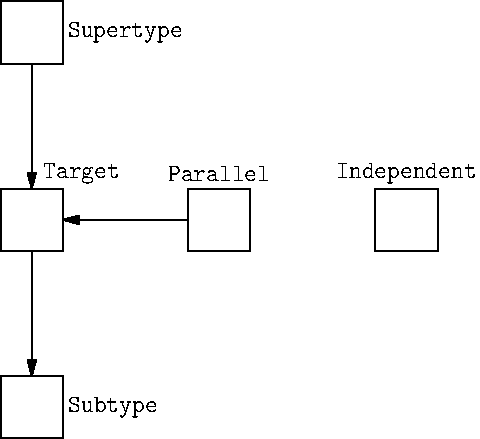
\includegraphics[width=0.5\textwidth]{typedef}
\caption{Typedef relationships}
\label{fig:typedef}
\end{figure}

\begin{description}
\item[subtype:] That's the standard subclass or \D{alias this} relationship: a subtype can act \emph{in lieu of} its parent type in all circumstances. Whatever its parent can do, the subtype does also. Moreover, the subtype can be forcibly cast as its parent type (think classes).
\item[supertype:] The converse: a supertype can be assigned a value of type 'target', its subtype (since a subtype can act as its supertype), and that's about it. Once the supertype and functions acting on it are created, the original target type can be used there also.
\item[parallel:] A parallel type is neither a subtype not a supertype of the original target (it cannot mimic the target), but it can be created with target values. It's more or less the behaviour of the now-deceased \D{typedef} keyword.
\item[independent:] An independent type is just there and bears no relationship whatsoever with the original, target type. I cite it there but the interest of defining such a type while still having a 'target' type in mind is limited\ldots
\end{description}

Here is clean little piece of code from Trass3r that groups all these notions in one template:

\begin{dcode}
module librarytypedef;

enum Relationship
{
    Independent,
    Super,
    Sub,
    Parallel,
}

struct Typedef( Target, 
                Relationship relation = Relationship.Sub, 
                Target init = Target.init, 
                string _f = __FILE__,
                int _l = __LINE__ )
{
    Target payload = init;

    static if ( relation != Relationship.Independent )
        this( Target value )
        {
            payload = value;
        }

    static if ( relation == Relationship.Sub)
        // typedef int foo; foo f;
        // f.opCast!(t)() == cast(t) f
        Target opCast(Target)()
        {
            return payload;
        }

    static if ( relation == Relationship.Sub 
             || relation == Relationship.Parallel )
        alias payload this;

    static if ( relation == Relationship.Super )
        typeof( this ) opAssign( Target value )
        {
            payload = value;
            return this;
        }
    else static if ( relation == Relationship.Sub )
        @disable void opAssign( Target value );
}
\end{dcode}

\TODO{Give some examples.}

\section{Types as Information}
\label{typesasinformation}

\subsection{User-Defined Literals}\label{userdefinedliterals}

In \href{http://drdobbs.com/blogs/tools/229401068}{this article}, Walter Bright makes a convincing case for using templates as user-defined literals. His example is now the \stdanchor{conv}{octal} wrapper that allowed D to (see if it's possible to) ditch octal literals as a compiler construct and push them into library-space. That way, you can use:

\begin{dcode}
auto o1 = octal!"755";
// or even:
auto o2 = octal!755;
\end{dcode}

as a stand-in replacement for the \DD{0755} octal literal. It's no more complicated to type (a few chars to add at most), it's clearer for a reader of your code (who may miss the beginning \DD{0}) that he's dealing with an octal there. Best of all, the implementation is there as library code: easy to reach, easy to debug\footnote{ And less intimidating than diving into compiler code.} and easy to duplicate for other encodings. That way, this could be done:

\begin{dcode}
auto h1 = hexa!"deadbeef";
auto b1 = binary!1011011;
// Or even:
auto number = base!(36, "4d6r7th2h7y");
\end{dcode}

Behind the scene, \DD{octal} reads its \D{string} or \D{int} argument and converts it into an \D{int} or a \D{long} depending on the argument size.  It's a nice piece of work that could pave the way to similar well-integrated language extensions.

\unfinished{Also, DSL in strings in D, see Statically-Checked Writeln in \ref{staticallycheckedwriteln}, encoding informations in types (\ref{encodinginformationwithtypes}) and annotating types (\ref{annotatingtypes}).}


\subsection{Encoding Information With Types}
\label{encodinginformationwithtypes}

This is an extension of the previous section's idea, that can be found for example in \stdanchor{range}{assumeSorted} and \stdanchor{range}{SortedRange}. These Phobos constructs encode some information in a type (in this case, the fact than the range is sorted, with an associated predicate). That way, subsequent operations acting on a range can use better algorithm if they know it's sorted.

This kind of encoding can be used for many different schemes:

\begin{itemize}
\item For a matrix library, you could have a, for example, \DD{assumeHermitian} or \DD{assumeTriangular} that just wraps a pre-existing matrix.
\item For a XML/HTML library, you could imagine a \DD{Validated} struct that's used to indicate, er, validated content. Any external input will have to pass trough a \DD{validate} function that delivers the \DD{Validated} object. Subsequent operations will work only on \DD{Validated} data, not raw data.
\item A units library (as in, $kg.m/s^{2}$, not unit-testing) is mainly a bunch of \D{double} (or complex) values wrapped in a multi-checked type that allows only some operations, depending on types. \DD{meter(5) + kilo(gram(10))} is a no-no, but \DD{meter(5)*kilo(gram(10))} is OK.
\end{itemize}

Moreover, it's easy to provide additional information:

\begin{dcode}
struct MinMax(T)
{
    T min;
    T max;
    
    T value;
    
    alias value this;
}
\end{dcode}

In this case, \DD{MinMax} means the wrapped value is between \DD{min} and \DD{max} (the enforcing code would be in the factory function, for example).
        
Things get interesting when using multiple wrappers inside one another. Imagine we have three wrappers, for numerical ranges with an ordering operation:

\begin{itemize}
\item \DD{minmaxed}, which ascertains (well, at least transmits the message) that the wrapped value is between to extrema.
\item \DD{periodic}, which encodes the idea the range has a period, accessible through the \DD{.period} member.
\item \DD{derivative}, which says successive elements' difference is no more than a \DD{.slope} number (in absolute).
\end{itemize}

\begin{dcode}
import std.range: cycle;

auto range = cycle([0,1,2,3,4,3,2,1]);
auto withMetadata = minmaxed( 
                              periodic( 
                                       derivative( range
                                                 , 1)
                                      , 8
                            , 0, 10);

assert(withMetadata.period == 8); // propagated all the way up.
\end{dcode}

So, in the previous sample, \DD{withMetadata}'s elements are at the same time limited in variation, limited in value and periodic. The trouble is when we want to shift metadata around, comparing types with metadata ordered in a different way: obviously for us humans, a range with suprema and periodic is \emph{also} periodic and with suprema. But as far as D is concerned a \DD{minmaxed(periodic())} and a \DD{periodic(minmaxed())} do not have the same type. For more on this notion, see section \ref{annotatingtypes} on annotating types.

\TODO{A unit example in the Examples part? It may be a bit big\ldots}

\section{Templates in Templates}\label{templatesintemplates}

Sometimes, you know users of your code will send to your template a first list (of indefinite length) of parameters, followed by a second list. Seeing that, you may want to write code like the following:

\begin{dcode}
template MyTemp(A..., B...)
{ ... }
\end{dcode}

Halas, two template parameters tuples do not make sense (see \autoref{declarations}). But it's not a dead-end. First, you could try to write:

\begin{dcode}
template(AB...)
{ ... }
\end{dcode}

And filter the \DD{AB}s to find the ones you need. It can be done by \DD{staticFilter}, presented in \ref{staticfilter} (and its associated function on a function arguments would be \DD{tupleFilter} shown in \ref{filteringtuples}). In this case, the two series of arguments can be completely mixed (and not separated in two lists), which is strictly more powerful. On the other hand, it means you must be able to separate them by their types alone, which may not be possible.

\subsection{Templates All the Way Down}

Happily, the initial problem can easily be solved this way:

\begin{dcode}
template MyTemp(A...)
{
    template MyTemp(B...)
    {
    (...)
    }
}
\end{dcode}

Remember, a template can have template members. So you can nest templates within templates, each with its own constraints and intermediate code. If you use the same name through and through the eponymous trick will be activated, but sometimes using a different name at each stage can make your code more readable.

For example, what if you want to compare to template tuples to see if they contain the same arguments?

\begin{dcode}
module compare;

template Compare(First...)
{
    template With(Second...)
    {
        static if (First.length != Second.length)
            enum With = false;
        else static if (First.length == 0) // End of comparison
            enum With = true;
        else static if (!is(First[0] == Second[0]))
            enum With = false;
        else
            enum With = Compare!(First[1..$]).With!(Second[1..$]);
    }
}

//Usage:
unittest
{
    alias Compare!(int, double, string).With!(int, double, char) C;
    static assert(C == false);
}
\end{dcode}

In that case, using \DD{With} inside \DD{Compare} let the code be quite easy to use. Notice that the eponymous trick is done only on \DD{With}, because it's this inner template that we want the result of.

Going back to \DD{MyTemp}, using it is slightly more complicated:

\begin{ndcode}
// Yes:
alias MyTemp!(int, double, string) MyTemp1;
MyTemp1!(char, void);

// No:
MyTemp!(int, double, string)!(char, void);
// No :
MyTemp!(int, double, string).!(char, void);
\end{ndcode}

The D grammar does not authorize multiple template calls like the ones on lines 6 and 8. You must use an alias for the intermediate stage. It's not that drastic a limitation, because if you created the template as a multi-step construction, it's most probably because you wanted to do a multi-step invocation\ldots

\subsection{Double-Stage Function Templates}

For function templates, this can give very powerful things. You can have a place in your code where compile-time parameters are given, which delivers another, crafted-just-for-your-needs, template which you can instantiate later on. See for example \ref{stringinterpolation} and the \DD{interpolate} function-in-template.

Policies are particularly good with this idiom.\index{idiom!functions in templates} Section \ref{memoizing} presents a template that transforms a standard D function into a memoized one. Here is what could be done if it was a two-steps template:

\begin{dcode}
/*
 * memoizer will store the first million tuple of args
 * and discard half of them when the maximum is reached, 
 * to free some memory. At this stage, the function it 
 * will memoize is not known. The user decided this
 * particular instantiation was the best memoizing 
 * strategy in her code. memoizer could (and will!) be 
 * applied on many different functions.
 */
alias memoize!(Storing.maximum, 1_000_000, Discarding.fraction, 0.5f) memoizer;

auto longCalculation1(int i, double d) { ... }
auto longCalculation2(double d, string s) { ... }

/*
 * longCalculation1 and longCalculation2 will both profit 
 * from the memoization even though they have different 
 * signatures, different arguments and return a different type.
 */
alias memoizer!longCalculation1 mlc1;
alias memoizer!longCalculation2 mlc2;
\end{dcode}

\TODO{OK, now maybe I should provide an updated version of \DD{memoize} in \ref{memoizing}.}

\subsection{Named-Fields Tuples}\label{namedfieldstuples}

Let's have another example, to use IFTI (\ref{ifti}). In Phobos, the function \stdanchor{typecons}{tuple} lets you create a tuple on the fly. It's a very nice example of IFTI in action:

\begin{dcode}
module usingtuple;
import std.typecons;

void main()
{
    auto tuple1 = tuple(1, 3.14159, "abc"); // tuple1 is a Tuple!(int,double,string)
    auto tuple2 = tuple('a','b','c');       // tuple2 is a Tuple!(char,char,char)
}
\end{dcode}

But Phobos' \DD{Tuple} is more powerful than that. It can have named parameters:

\begin{dcode}
Tuple!(int, "counter", string, "name") myCounter;
myCounter.counter = -1;
myCounter.name = "The One and Only Counter Around There";
\end{dcode}

As of this writing, Phobos doesn't provide a \DD{tuple} factory function allowing named arguments in an nice, automated manner:

\begin{dcode}
module usingnamedtuple;
import namedtuple;

void main()
{
    auto myCounter = tuple!("counter", "name")(-1, "Who's his Daddy's counter?");

    myCounter.counter = 1;

    // Or even:
    alias tuple!("counter", "name") makeCounter;

    auto c1 = makeCounter(0, "I count ints!");
    auto c2 = makeCounter("Hello", "I'm a strange one, using strings");

    c2.counter ~= " World!"; 
}
\end{dcode}

In the previous example, \DD{c1} is a \DD{Tuple!(}\D{int}\DD{,}\D{string}\DD{)}, whereas \DD{c2} is a \DD{Tuple!(}\D{string}\DD{,}\D{string}\DD{)}. That means \DD{makeCounter} is a factory function for tuples with two fields, named \DD{counter} and \DD{name}, which see their types determined later on. I want this, so let's code it.

First, it's obvious we need a two-stage template:

\index{template!constraints}
\begin{dcode}
import std.typetuple: allSatisfy;

template tuple(names...) 
if (names.length && allSatisfy!(isAStringLiteral, names))
{
    auto tuple(T...)(T args)
    {
    (...)
    }
}
\end{dcode}

The constraint is here to check that the user gives at least one name and also that all passed \DD{names} are indeed string literals template parameters. I use \stdanchor{typetuple}{allSatisfy} to verify the condition on all of them. I cannot use directly \stdanchor{traits}{isSomeString} because this template acts on types, whereas I need something checking a string literal.

\begin{dcode}
module isastringliteral;
import std.traits: isSomeString;

template isAStringLiteral(alias name)
{
    enum isAStringLiteral = isSomeString!(typeof(name));
}
\end{dcode}

That being in place, we need to create the correct \DD{Tuple}. Arguments names are provided right after each type (so as to allow for a mix between named and anonymous fields:

\begin{dcode}
/*
 * The first two fields are named, and the fourth.
 * The third is anonymous.
 */
alias Tuple!(int, "counter", string, "name", double, double, "total") MyTuple;
\end{dcode}

For our function, we consider that, given $n$ names, the first $n$ arguments will be named and the remaining (if any) will be anonymous. That give us another constraint: if the user provide less than $n$ arguments, we refuse the input and stop the compilation right there.

\index{template!constraints}
\begin{dcode}
import std.typetuple: allSatisfy;

template tuple(names...) 
if (names.length && allSatisfy!(isAStringLiteral, names))
{
    auto tuple(T...)(T args) if (T.length >= names.length)
    {
    (...)
    }
}
\end{dcode}

Now, we just need the alternate the names and the argument types. Happily, this document describe a \DD{Interleave} template in \ref{interleavingtypes}, that does just that:

\begin{dcode}
module namedtuple;
import std.typecons;
import std.typetuple;
import interleave;
import isastringliteral;

template tuple(names...) 
if (names.length && allSatisfy!(isAStringLiteral, names))
{
    auto tuple(T...)(T args) if (T.length >= names.length)
    {
        return Tuple!(Interleave!(T).With!(names))(args);
    }
}
\end{dcode}

And, presto, here we have our named-tuple factory function. Isn't that nice? The closure example in \ref{closuresareapoormansobjects} could use it to simplify its returned value.

\TODO{And a curried template.}

\section{\texorpdfstring{\D{\_\_FILE\_\_} and \D{\_\_LINE\_\_}}
                        {\_\_FILE\_\_ and \_\_LINE\_\_}}
\label{fileandline}

\unfinished{This section needs some heavy testing. My D config was broken when I wrote this part. Take everything in there with a \emph{big} grain of salt. It's on my todo list to test and rewrite everything.}

In section \ref{default}, we've seen that template parameters can have default values. There are also two special, reserved, symbols that are defined in D: \D{\_\_FILE\_\_} and \D{\_\_LINE\_\_}. They are used in standard (non-\D{mixin}) templates, but their behaviour will remind you of mixins: when instantiated, they get replaced by strings containing the file name and the line in the file of the \emph{instantiation call site}. Yes, it's a sort of two-way dialogue: module \DD{a.d} defines template \DD{T}. Module \DD{b.d} asks for a \DD{T} instantiation. This instantiation is done in module \DD{a.d}, but will line and filename taken from \DD{b.d}!

They are mostly declared like this:

\index{\_\_FILE\_\_ and \_\_LINE\_\_@\D{\_\_FILE\_\_} and \D{\_\_LINE\_\_}!unique types}
\begin{dcode}
module filelinetagging;

struct Unique(T, string file, size_t line)
{
    enum size_t l = line;
    enum string f = file;
    T t;
}

auto unique(T, string file = __FILE__, size_t line = __LINE__)(T t)
{
    return Unique!(T, file, line)(t);
}
\end{dcode}

As \DD{Unique}'s name suggests, this is a way to obtain unique instantiations. Except if you call the very same template twice in the same line of your file, this pretty much guarantee your instantiation will be the only one. Remember that template arguments become part of the template scope\index{scope!template scope} name when instantiation is done (\ref{instantiating}).

\begin{dcode}
module usingunique;
import filelinetagging;

void main()
{
    auto u = unique(1); // Unique!(int, "thefile.d", 4)

    auto v = unique(1); // Unique!(int, "thefile.d", 6)

    static assert(!is( typeof(v) == typeof(u) ));
}
\end{dcode}

Even though \DD{u} and \DD{v} are declared the same way, they have different types.

Apart from \emph{one-of-a-kind} types, this is also useful for debugging: you can use the strings in error messages:

\index{\_\_FILE\_\_ and \_\_LINE\_\_@\D{\_\_FILE\_\_} and \D{\_\_LINE\_\_}!debugging}
\begin{dcode}
auto flatten(Range, file == __FILE__, line == __LINE__)(Range range)
{ 
    static if (rank!Range == 0)
        static assert(0, "File: " ~ file ~ " at line: " ~ line 
                       ~ ", flatten called with a rank-0 type: " 
                       ~ Range.stringof);
    else static if (rank!Range == 1)
        return range;
    else
        return Flatten!(Range)(range);
}
\end{dcode}

And here is a little gift:

\begin{dcode}
module debugger;

/** Usage:
 * Debug!(templateToBeTested).With!(Argument0, Argument1, Argument2);
 */
template Debug(alias toTest, string file = __FILE__, size_t line = __LINE__)
{
    template With(Args...)
    {
        static if (is( toTest!Args ))
            alias toTest!Args With;
        else
            static assert(0, "Error: " ~ to!string(toTest)
                           ~ " called withs arguments: "
                           ~ Args.stringof);
    }
}
\end{dcode}

That way, no need to modify your beautiful templates.

\TODO{Test that.}


